%%%%%%%%%%%%%%%%%%%%%%%%%%%%%%%%%%%%%%%%%%%%%%%%%%%%%%%%%%%%%%%%%%%%%%%%%%%%%%%%
%2345678901234567890123456789012345678901234567890123456789012345678901234567890
%        1         2         3         4         5         6         7         8

\documentclass[letterpaper, 10 pt, conference]{ieeeconf}  % Comment this line out
                                                          % if you need a4paper
%\documentclass[a4paper, 10pt, conference]{ieeeconf}      % Use this line for a4
                                                          % paper

\IEEEoverridecommandlockouts                              % This command is only
                                                          % needed if you want to
                                                          % use the \thanks command
\overrideIEEEmargins
% See the \addtolength command later in the file to balance the column lengths
% on the last page of the document



% The following packages can be found on http:\\www.ctan.org
\usepackage{graphicx} % for pdf, bitmapped graphics files
%\usepackage{epsfig} % for postscript graphics files
%\usepackage{mathptmx} % assumes new font selection scheme installed
%\usepackage{times} % assumes new font selection scheme installed
%\usepackage{amsmath} % assumes amsmath package installed
%\usepackage{amssymb}  % assumes amsmath package installed
\usepackage{indentfirst}

\title{\LARGE \bf
Client-Server Application for Storage Administering of Source Code Change Patterns
}

\author{
Alexander Krasnov \\ 
\textit{Faculty of Computer Science, Higher School of Economics} \\
Moscow, Russia \\
aakrasnov@edu.hse.ru
}


\begin{document}


\maketitle
\thispagestyle{empty}
\pagestyle{empty}

%%%%%%%%%%%%%%%%%%%%%%%%%%%%%%%%%%%%%%%%%%%%%%%%%%%%%%%%%%%%%%%%%%%%%%%%%%%%%%%%
\begin{abstract}

Modern software projects are extremely complex: they contain thousands of lines
of code and use a large number of third-party libraries.
Their maintenance is a highly laborious task, which includes a number of
repetitive actions based on source code changes of a certain type (library
migrations, common bug fixes, rule-based refactoring, etc.).
One of the ways to improve the efficiency of software developers is to
automate such changes using a pattern-based approach. 
Patterns are editing scripts based on an abstract syntax tree, which are 
mined from a history of manual changes and are stored in documents of a 
special format. 
The collection of patterns covering possible change scenarios is constantly
increasing.
An important task is to organise a centralised storage of documents with
patterns and their distribution to users. 
The storage must provide the possibility to collect a feedback from users, 
which will be used to improve pattern quality. 
This task has not been solved yet as modern pattern-mining tools are research
projects that are on the way of becoming industrial products.
This paper describes a client-server application for storage administering of
source code change patterns and their usage statistics.
\end{abstract}

\begin{keywords} 
storage, patterns, library migration, administering
\end{keywords}


%%%%%%%%%%%%%%%%%%%%%%%%%%%%%%%%%%%%%%%%%%%%%%%%%%%%%%%%%%%%%%%%%%%%%%%%%%%%%%%%
\section{Introduction}
During the project lifecycle, developers often face the following
typical tasks: replacing used libraries, correcting common errors,
and restructuring the code according to certain rules \cite{c4}. 
Completing these tasks is time-consuming and error-prone, although it is
possible to automate this process by applying \emph{patterns} based on an
\emph{abstract syntax tree} (AST) \cite{c1, c2, c3}. 
Automation of routine actions using templates will increase the productivity of
developers and the quality of the project source code.

The obvious questions that arise in this case are where to store and
how to distribute these changes. 
For this purpose a \emph{central storage} will be developed. 
It is expected that templates can come from different sources and be specific
to a project (for example, a pet project) or a group of projects. 
Moreover, the set of patterns will be constantly updated. 
These assumptions contribute to provide an opportunity for storing templates,
updating them and leaving feedback about the usage of existing ones.

The following \emph{requirements} apply to the application being developed:
\begin{enumerate}
    \item It must store patterns which are combined into \emph{documents}
    with the addition of metadata information.
    \item It must also be possible to get, put, search and
    update patterns.
    \item A user must be able to leave a feedback about the usage of
    downloaded documents.
    \item The system administrator must have an opportunity to set limits on
    the number of uploaded patterns.
\end{enumerate}

The remainder of the paper is organised in a following way. 
In Section~\ref{section:review} related literature is reviewed. 
In Section~\ref{section:method}, the methodology is described. 
Section~\ref{section:results} contains discussion about the expected results.
The last Section~\ref{section:conclusion} summarises the paper.

\section{Literature review}
\label{section:review}

The concept of pattern-based tools is described in works \cite{c1, c2, c3}.
The main idea is to \emph{mine} AST-based patterns from a history of 
changes (e.g. by browsing commits in open-source project repositories) and 
apply them to repeat the changes in other source code files that contain
matching fragments. 
Patterns are minimised and generalis    ed AST subtrees with editing actions
(delete, insert and update) \cite{c9} that describe the changes to be applied.

The task of storing and distributing patterns is not discussed in existing
publications. 
This can be explained by the fact that pattern-based code fixers are research
projects which currently do not have a large community of users. 
However, the centralised pattern repository will be an important component
for a commercial product.

The first thing to consider when designing a storage system is the storage
format. 
Firstly, it must be a human-readable format that is suitable for
representing AST-based data. 
Secondly, it must be compact and appropriate for transferring over a network 
using a REST (Representational State Transfer) protocol. 
Thirdly, it must be suitable for storing complex structured data.
JSON (JavaScript Object Notation) \cite{c7} is the format that meets mentioned
requirements.
Many code parsing tools such as Clang and JavaParser~\cite{c8} serialize 
their ASTs in JSON. 
Also, pattern-based tool Patternika~\cite{c1} created by Huawei company uses
JSON as its input and output formats.
Finally, many REST services are based on JSON and there are many high-quality
libraries available for serializing/deserializing JSON. 
Considering the above advantages, JSON is chosen as the data storage format.

As for architecture, client-server applications allow to divide data
processing responsibilities between the server and the client. 
To be more precise, the serialization of data is assigned to the client. 
In addition, it is possible to send requests to the service with different
filters, and apply these filters on the server side. 
This separation of chores gives an opportunity to reduce the load on the
network, which generally contributes to improving the performance of the
application \cite{c10}. 
According to comparison (relational model VS document-oriented model)
\cite{c11}, it is decided to use NoSQL database as it meets a requirement 
to store documents with patterns in document-oriented format. 
In addition, the strong points of databases of this type are the ability to
scale and store quite large amounts of data.

\section{Methodology}
\label{section:method}

The main idea is to work out a centralised storage which will contain AST-based
patterns describing source code changes.
The whole workflow looks in a following way.
Developers create different examples of patterns using the approaches described
in the previous section.
After that users must be authenticated in order to upload mined patterns and
have to comply with the set limits to be able to perform this operation.
They should specify metadata information to create a new document with these
patterns.
In the next step, users can download these documents.
The Figure~\ref{fig:architecture} specifies the common architecture of the
application.
There is a \emph{service} which connects to the \emph{database} and processes
request from clients. 
A \emph{client} part provides the list of required functions to interact 
with patterns, whereas an ordinary user can use these functions via 
\emph{Web UI} or \emph{CLI}.

\begin{figure}[hbtp]
    \centerline{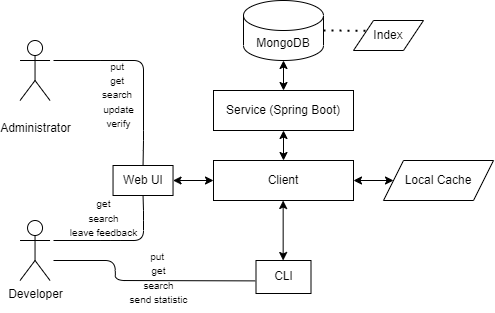
\includegraphics[width=0.52\textwidth]{arch}}
    \caption{Client-server application architecture.}
    \label{fig:architecture}
\end{figure}

\subsection{Server}
In general patterns are useful only in the case of using a certain set of them.
For this purpose they are combined into documents which contain some metadata
information.
It includes a unique identifier, the name of the programming language for which
this document is used, as well as the application scenario. 
This scenario contains type of information (migration, refactoring or an unknown
type), whereas each pattern also has several descriptive fields, which allow 
to identify it.
Moreover, it is possible to get information about the creation time, the author
of the pattern and some specific metadata.

As for the administrator of the system, he/she can limit the number of uploaded
patterns, specify some restrictions for the maximum amount of uploaded data 
or just prohibit the upload to a specific user. 
Another available functionality for the administrator is an opportunity to
modify existing documents by merging some of them, updating and deleting them.

Spring is used as a framework for the development of a standalone 
application \cite{c5}.
MongoDB is used as a document-oriented database management system \cite{c6}. 

\subsection{Client}
The most common way of using the service is to download existing documents 
from the storage. 
A user has several filters to obtain only necessary documents with patterns. 
For example, he can specify the full description of the library to be replaced
during migration, and the same for the library which will update the previous
one. 
Another available filter is to get all the data for a specific programming
language. 
After downloading documents from a centralised repository, patterns are 
applied using the Patternika tool \cite{c1}. 

\subsection{Cache}
Asking for upload of the same documents is quite common for the process of
applying patterns from them, therefore it is decided to develop a 
\emph{local client cache}. 
Further details of the operation of the cache will be given here:
\begin{itemize}
    \item It must be able to get a document from the local cache, if there
    is no connection to the service and the necessary item exists.
    \item If the service is available and the item exists in the
    local memory, it is necessary to check that the data has not expired
    (for example, the local timestamp of the document and the timestamp of
    the deleted document match).
    \item If cached documents have been modified locally in some way
    and these changes have been transferred to the service, such documents
    should be deleted from the local cache.
    \item There is no need to validate the local cache very often.
    A document can be considered fresh (e.g. not expired) if it is
    updated within the specified time interval (for example, 1 hour).
    Immediate refreshing of documents is not critical. 
    It is better to avoid redundant requests to the server.
\end{itemize}

\section{Expected results}
\label{section:results}

The desired result of this work is a client-server application which
meets mentioned above requirements. 
It allows to distribute and store patterns.
An ordinary user will search for documents with patterns and download them
without authentication, whereas only authenticated users will be able to 
upload new patterns to the repository. 
Uploaded patterns will be stored and passed in JSON format in the repository.
In addition, a local client cache will be implemented.
As for the administrator of the system, he/she will have the opportunity to
limit the available number of uploads per user and to merge and update 
patterns in the documents. 

\section{Conclusion}
\label{section:conclusion}

Automation of modifying source code is becoming more popular in the world of
software development as it allows to reduce the amount of monotonous work. 
This helps to improve the quality of the source code and reduce the
influence of the human factor on the occurrence of errors. 
Following these trends, the number of patterns increases, covering more 
and more cases. 
In this paper, it is proposed to develop a centralised repository with 
patterns to distribute them among different teams and developers. 
A client-server application with the opportunity of administering it is the
target of this work.

\addtolength{\textheight}{-12cm}   % This command serves to balance the column lengths
                                  % on the last page of the document manually. It shortens
                                  % the textheight of the last page by a suitable amount.
                                  % This command does not take effect until the next page
                                  % so it should come on the page before the last. Make
                                  % sure that you do not shorten the textheight too much.

%%%%%%%%%%%%%%%%%%%%%%%%%%%%%%%%%%%%%%%%%%%%%%%%%%%%%%%%%%%%%%%%%%%%%%%%%%%%%%%%



%%%%%%%%%%%%%%%%%%%%%%%%%%%%%%%%%%%%%%%%%%%%%%%%%%%%%%%%%%%%%%%%%%%%%%%%%%%%%%%%



%%%%%%%%%%%%%%%%%%%%%%%%%%%%%%%%%%%%%%%%%%%%%%%%%%%%%%%%%%%%%%%%%%%%%%%%%%%%%%%%



\begin{thebibliography}{99}
\bibitem{c4} C. Teyton, J. Falleri, M. Palyart, and X. Blanc, “A study of
library migration in java software,” 2013.
\bibitem{c1} Andrei Tatarnikov et al., “Patternika: A
Pattern-Mining-Based Tool for Automatic Library Migration”,
Proceedings of the 32nd International Symposium on Software
Reliability Engineering (ISSRE 2021), Wuhan, China, 2021, p. 6.
\bibitem{c2} J. Bader, A. Scott, M. Pradel, and S. Chandra, “Getafix:
Learning to fix bugs automatically”, Proceedings of the ACM on Programming
Languages, p. 19, 2019.
\bibitem{c3} R. Rolim, G. Soares, R. Gheyi, and L. D’Antoni, “Learning
quick fixes from code repositories,” p. 12, 2018.
\bibitem{c5} Spring Development Team. (2022). Spring Boot Reference
Documentation. Retrieved from
https://docs.spring.io/spring-boot/docs/current/reference/pdf/spring-boot-reference.pdf
\bibitem{c6} MongoDB Development Team. (2022). Retrieved from
https://docs.mongodb.com/manual/
\bibitem{c7} JSON format. Retrieved from https://en.wikipedia.org/wiki/JSON
\bibitem{c8} Nicholas Smith, Danny van Bruggen, and Federico Tomassetti
(2021). JavaParser: Visited. Retrieved from
https://leanpub.com/javaparservisited
\bibitem{c9} Jean-Rémy Falleri et al. Fine-grained and Accurate Source Code
Differencing. Proceedings of the International Conference on Automated
Software Engineering, 2014, Västeras, Sweden. pp.313-324. Retrieved from
https://hal.inria.fr/hal-01054552
\bibitem{c10} UKEssays. (2018). Client Server Network Architecture Essay.
Retrieved from https://www.ukessays.com/essays/computer-science/client-server-architecture.php
\bibitem{c11} Kleppmann, M. (2017). Designing Data-Intensive Applications (pp.
53-70). Beijing: O'Reilly. ISBN: 978-1-4493-7332-0
\bibitem{c12} REST protocol. Retrieved from
https://en.wikipedia.org/wiki/REST
\end{thebibliography}
\end{document}
